\documentclass[twoside]{book}

% Packages required by doxygen
\usepackage{fixltx2e}
\usepackage{calc}
\usepackage{doxygen}
\usepackage{graphicx}
\usepackage[utf8]{inputenc}
\usepackage{makeidx}
\usepackage{multicol}
\usepackage{multirow}
\PassOptionsToPackage{warn}{textcomp}
\usepackage{textcomp}
\usepackage[nointegrals]{wasysym}
\usepackage[table]{xcolor}

% NLS support packages
\usepackage[french]{babel}

% Font selection
\usepackage[T1]{fontenc}
\usepackage{mathptmx}
\usepackage[scaled=.90]{helvet}
\usepackage{courier}
\usepackage{amssymb}
\usepackage{sectsty}
\renewcommand{\familydefault}{\sfdefault}
\allsectionsfont{%
  \fontseries{bc}\selectfont%
  \color{darkgray}%
}
\renewcommand{\DoxyLabelFont}{%
  \fontseries{bc}\selectfont%
  \color{darkgray}%
}
\newcommand{\+}{\discretionary{\mbox{\scriptsize$\hookleftarrow$}}{}{}}

% Page & text layout
\usepackage{geometry}
\geometry{%
  a4paper,%
  top=2.5cm,%
  bottom=2.5cm,%
  left=2.5cm,%
  right=2.5cm%
}
\tolerance=750
\hfuzz=15pt
\hbadness=750
\setlength{\emergencystretch}{15pt}
\setlength{\parindent}{0cm}
\setlength{\parskip}{0.2cm}
\makeatletter
\renewcommand{\paragraph}{%
  \@startsection{paragraph}{4}{0ex}{-1.0ex}{1.0ex}{%
    \normalfont\normalsize\bfseries\SS@parafont%
  }%
}
\renewcommand{\subparagraph}{%
  \@startsection{subparagraph}{5}{0ex}{-1.0ex}{1.0ex}{%
    \normalfont\normalsize\bfseries\SS@subparafont%
  }%
}
\makeatother

% Headers & footers
\usepackage{fancyhdr}
\pagestyle{fancyplain}
\fancyhead[LE]{\fancyplain{}{\bfseries\thepage}}
\fancyhead[CE]{\fancyplain{}{}}
\fancyhead[RE]{\fancyplain{}{\bfseries\leftmark}}
\fancyhead[LO]{\fancyplain{}{\bfseries\rightmark}}
\fancyhead[CO]{\fancyplain{}{}}
\fancyhead[RO]{\fancyplain{}{\bfseries\thepage}}
\fancyfoot[LE]{\fancyplain{}{}}
\fancyfoot[CE]{\fancyplain{}{}}
\fancyfoot[RE]{\fancyplain{}{\bfseries\scriptsize Généré le Vendredi 20 Février 2015 16\+:01\+:46 pour Bot Sushi Go Round par Doxygen }}
\fancyfoot[LO]{\fancyplain{}{\bfseries\scriptsize Généré le Vendredi 20 Février 2015 16\+:01\+:46 pour Bot Sushi Go Round par Doxygen }}
\fancyfoot[CO]{\fancyplain{}{}}
\fancyfoot[RO]{\fancyplain{}{}}
\renewcommand{\footrulewidth}{0.4pt}
\renewcommand{\chaptermark}[1]{%
  \markboth{#1}{}%
}
\renewcommand{\sectionmark}[1]{%
  \markright{\thesection\ #1}%
}

% Indices & bibliography
\usepackage{natbib}
\usepackage[titles]{tocloft}
\setcounter{tocdepth}{3}
\setcounter{secnumdepth}{5}
\makeindex

% Hyperlinks (required, but should be loaded last)
\usepackage{ifpdf}
\ifpdf
  \usepackage[pdftex,pagebackref=true]{hyperref}
\else
  \usepackage[ps2pdf,pagebackref=true]{hyperref}
\fi
\hypersetup{%
  colorlinks=true,%
  linkcolor=blue,%
  citecolor=blue,%
  unicode%
}

% Custom commands
\newcommand{\clearemptydoublepage}{%
  \newpage{\pagestyle{empty}\cleardoublepage}%
}


%===== C O N T E N T S =====

\begin{document}

% Titlepage & ToC
\hypersetup{pageanchor=false,
             bookmarks=true,
             bookmarksnumbered=true,
             pdfencoding=unicode
            }
\pagenumbering{roman}
\begin{titlepage}
\vspace*{7cm}
\begin{center}%
{\Large Bot Sushi Go Round }\\
\vspace*{1cm}
{\large Généré par Doxygen 1.8.8}\\
\vspace*{0.5cm}
{\small Vendredi 20 Février 2015 16:01:46}\\
\end{center}
\end{titlepage}
\clearemptydoublepage
\tableofcontents
\clearemptydoublepage
\pagenumbering{arabic}
\hypersetup{pageanchor=true}

%--- Begin generated contents ---
\chapter{mini\+Projet\+Sush\+Go\+Round}
\label{md_README}
\hypertarget{md_README}{}
Mini Projet 2015 Université Paris-\/\+Sud

Sujet\+:

Créer une mini-\/\+I\+A pour jour à \href{http://www.miniclip.com/games/sushi-go-round/en/}{\tt Sushi Go Round}

Equipe\+:

Dimitri Belopopsky Sofiane Adjiri Antoine Dolant Raphaël Cohen 
\chapter{Index des classes}
\section{Liste des classes}
Liste des classes, structures, unions et interfaces avec une brève description \+:\begin{DoxyCompactList}
\item\contentsline{section}{\hyperlink{classFindPicture}{Find\+Picture} \\*\mbox{[}brief description\mbox{]} }{\pageref{classFindPicture}}{}
\item\contentsline{section}{\hyperlink{classGame}{Game} \\*Classe qui s'occupe de gérer le jeu à jouer et initialiser l'I.\+A }{\pageref{classGame}}{}
\item\contentsline{section}{\hyperlink{classProg}{Prog} }{\pageref{classProg}}{}
\item\contentsline{section}{\hyperlink{classScreen}{Screen} \\*\mbox{[}brief description\mbox{]} }{\pageref{classScreen}}{}
\item\contentsline{section}{\hyperlink{classScreenCaptureRectangle}{Screen\+Capture\+Rectangle} \\*Classe pour créer les screenshots nécessaire au jeu }{\pageref{classScreenCaptureRectangle}}{}
\end{DoxyCompactList}

\chapter{Documentation des classes}
\hypertarget{classFindPicture}{\section{Référence de la classe Find\+Picture}
\label{classFindPicture}\index{Find\+Picture@{Find\+Picture}}
}


\mbox{[}brief description\mbox{]}  




Graphe de collaboration de Find\+Picture\+:\nopagebreak
\begin{figure}[H]
\begin{center}
\leavevmode
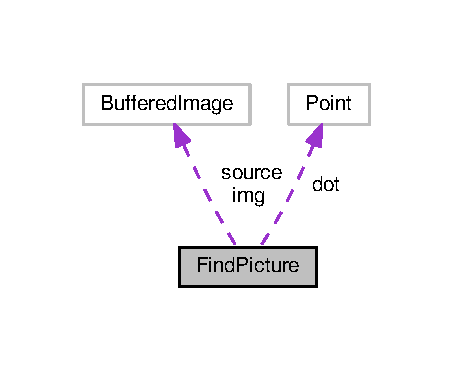
\includegraphics[width=218pt]{classFindPicture__coll__graph}
\end{center}
\end{figure}
\subsection*{Fonctions membres publiques}
\begin{DoxyCompactItemize}
\item 
\hyperlink{classFindPicture_ad697aff71f6479cf2345e6a80ed4ebb6}{Find\+Picture} (Buffered\+Image src, String img)
\begin{DoxyCompactList}\small\item\em constructeur on doit donc y mettre une buffered image qui sera le screen et le path du sprite à chercher \end{DoxyCompactList}\item 
\hypertarget{classFindPicture_a2204f21029e624f020162403c1575b47}{void {\bfseries load\+Pictures} (String path\+Img)}\label{classFindPicture_a2204f21029e624f020162403c1575b47}

\item 
\hypertarget{classFindPicture_aac2aafb41b291a82a8610a04c1025ce1}{Array\+List$<$ Integer $>$ {\bfseries get\+Line} (Buffered\+Image img, int line)}\label{classFindPicture_aac2aafb41b291a82a8610a04c1025ce1}

\item 
\hypertarget{classFindPicture_ac2dd2bde3776151960bff136fea75dc6}{Array\+List$<$ Integer $>$ {\bfseries get\+Column} (Buffered\+Image img, int column)}\label{classFindPicture_ac2dd2bde3776151960bff136fea75dc6}

\item 
\hypertarget{classFindPicture_aabc9cdcfadd7342e9f961d62f87997d0}{boolean {\bfseries check\+Column} (Buffered\+Image source, Buffered\+Image img)}\label{classFindPicture_aabc9cdcfadd7342e9f961d62f87997d0}

\item 
\hypertarget{classFindPicture_aa7bb6bab2d2cdebbacf9b6dadebad78b}{boolean {\bfseries check\+Line} (Buffered\+Image source, Buffered\+Image img)}\label{classFindPicture_aa7bb6bab2d2cdebbacf9b6dadebad78b}

\item 
\hypertarget{classFindPicture_ae170b7d5206ef838e49ab18dd2f930ac}{Buffered\+Image {\bfseries get\+Src} ()}\label{classFindPicture_ae170b7d5206ef838e49ab18dd2f930ac}

\item 
\hypertarget{classFindPicture_a74227c37722d2af2338a10da9bf97847}{Buffered\+Image {\bfseries get\+Img} ()}\label{classFindPicture_a74227c37722d2af2338a10da9bf97847}

\item 
\hypertarget{classFindPicture_a97f9a07435e5d763ebc17410a96a108f}{int {\bfseries get\+X} ()}\label{classFindPicture_a97f9a07435e5d763ebc17410a96a108f}

\item 
\hypertarget{classFindPicture_aeb910c0c9658a3dd341df9c502a09954}{int {\bfseries get\+Y} ()}\label{classFindPicture_aeb910c0c9658a3dd341df9c502a09954}

\end{DoxyCompactItemize}
\subsection*{Fonctions membres publiques statiques}
\begin{DoxyCompactItemize}
\item 
\hypertarget{classFindPicture_a882f95d8fa03bbacf268c946a5f8ff47}{static void {\bfseries main} (String\mbox{[}$\,$\mbox{]} args)  throws A\+W\+T\+Exception}\label{classFindPicture_a882f95d8fa03bbacf268c946a5f8ff47}

\end{DoxyCompactItemize}
\subsection*{Attributs publics}
\begin{DoxyCompactItemize}
\item 
\hypertarget{classFindPicture_a903eebbadc58375a46271ff8bd42d720}{Buffered\+Image {\bfseries source}}\label{classFindPicture_a903eebbadc58375a46271ff8bd42d720}

\item 
\hypertarget{classFindPicture_a2a40b15a3659e303de831714005d675b}{Point {\bfseries dot}}\label{classFindPicture_a2a40b15a3659e303de831714005d675b}

\end{DoxyCompactItemize}


\subsection{Description détaillée}
\mbox{[}brief description\mbox{]} 

\mbox{[}long description\mbox{]}


\begin{DoxyParams}{Paramètres}
{\em src} & \mbox{[}description\mbox{]} \\
\hline
{\em img} & \mbox{[}description\mbox{]}\\
\hline
\end{DoxyParams}
\begin{DoxyReturn}{Renvoie}
\mbox{[}description\mbox{]} 
\end{DoxyReturn}


\subsection{Documentation des constructeurs et destructeur}
\hypertarget{classFindPicture_ad697aff71f6479cf2345e6a80ed4ebb6}{\index{Find\+Picture@{Find\+Picture}!Find\+Picture@{Find\+Picture}}
\index{Find\+Picture@{Find\+Picture}!Find\+Picture@{Find\+Picture}}
\subsubsection[{Find\+Picture}]{\setlength{\rightskip}{0pt plus 5cm}Find\+Picture.\+Find\+Picture (
\begin{DoxyParamCaption}
\item[{Buffered\+Image}]{src, }
\item[{String}]{img}
\end{DoxyParamCaption}
)}}\label{classFindPicture_ad697aff71f6479cf2345e6a80ed4ebb6}


constructeur on doit donc y mettre une buffered image qui sera le screen et le path du sprite à chercher 

\mbox{[}long description\mbox{]}


\begin{DoxyParams}{Paramètres}
{\em src} & \hyperlink{classScreen}{Screen} du jeu en cours \\
\hline
{\em img} & Chemin de l'image à trouver \\
\hline
\end{DoxyParams}


La documentation de cette classe a été générée à partir du fichier suivant \+:\begin{DoxyCompactItemize}
\item 
Find\+Picture.\+java\end{DoxyCompactItemize}

\hypertarget{classGame}{\section{Référence de la classe Game}
\label{classGame}\index{Game@{Game}}
}


Classe qui s'occupe de gérer le jeu à jouer et initialiser l'I.\+A.  


\subsection*{Fonctions membres publiques}
\begin{DoxyCompactItemize}
\item 
\hyperlink{classGame_a573ef60b3a39bf46b372d8b0934288c3}{Game} (String url)
\begin{DoxyCompactList}\small\item\em Initialise le jeu à jouer ainsi que l'I\+A. \end{DoxyCompactList}\item 
Buffered\+Image \hyperlink{classGame_ae01d0cebaa4cac6dba20772e5fc74eb3}{get\+Screen} (int x)
\begin{DoxyCompactList}\small\item\em Méthode qui prend un screen après x temps. \end{DoxyCompactList}\item 
Buffered\+Image \hyperlink{classGame_acbe5038734e186ae2b049fbace6a62e2}{get\+Screen} ()
\begin{DoxyCompactList}\small\item\em Méthode qui prend la partie de l'écran qui détient le jeu. \end{DoxyCompactList}\item 
void \hyperlink{classGame_a7f6dd2359a96d4f725a727729e63a738}{create\+Screen\+Image} (Buffered\+Image image)
\begin{DoxyCompactList}\small\item\em Méthode qui prend une image et l'enregistre en P\+N\+G. \end{DoxyCompactList}\item 
void \hyperlink{classGame_a0f1d4ce523a41d2c3e275fe7478d1baa}{Start} (String src\+Path)  throws A\+W\+T\+Exception
\begin{DoxyCompactList}\small\item\em \mbox{[}brief description\mbox{]} \end{DoxyCompactList}\end{DoxyCompactItemize}
\subsection*{Fonctions membres publiques statiques}
\begin{DoxyCompactItemize}
\item 
\hypertarget{classGame_ae52595a27ac1b327b05db2129ad81fca}{static void {\bfseries main} (String\mbox{[}$\,$\mbox{]} args)}\label{classGame_ae52595a27ac1b327b05db2129ad81fca}

\end{DoxyCompactItemize}


\subsection{Description détaillée}
Classe qui s'occupe de gérer le jeu à jouer et initialiser l'I.\+A. 

\mbox{[}long description\mbox{]} 

\subsection{Documentation des constructeurs et destructeur}
\hypertarget{classGame_a573ef60b3a39bf46b372d8b0934288c3}{\index{Game@{Game}!Game@{Game}}
\index{Game@{Game}!Game@{Game}}
\subsubsection[{Game}]{\setlength{\rightskip}{0pt plus 5cm}Game.\+Game (
\begin{DoxyParamCaption}
\item[{String}]{url}
\end{DoxyParamCaption}
)}}\label{classGame_a573ef60b3a39bf46b372d8b0934288c3}


Initialise le jeu à jouer ainsi que l'I\+A. 

\mbox{[}long description\mbox{]}


\begin{DoxyParams}{Paramètres}
{\em url} & L'url du jeu à lancer (Exemple\+: \char`\"{}http\+://www.\+jeux-\/flash-\/gratuits.\+biz/games/sushi-\/go-\/round.\+swf\char`\"{}) \\
\hline
\end{DoxyParams}


\subsection{Documentation des fonctions membres}
\hypertarget{classGame_a7f6dd2359a96d4f725a727729e63a738}{\index{Game@{Game}!create\+Screen\+Image@{create\+Screen\+Image}}
\index{create\+Screen\+Image@{create\+Screen\+Image}!Game@{Game}}
\subsubsection[{create\+Screen\+Image}]{\setlength{\rightskip}{0pt plus 5cm}void Game.\+create\+Screen\+Image (
\begin{DoxyParamCaption}
\item[{Buffered\+Image}]{image}
\end{DoxyParamCaption}
)}}\label{classGame_a7f6dd2359a96d4f725a727729e63a738}


Méthode qui prend une image et l'enregistre en P\+N\+G. 


\begin{DoxyParams}{Paramètres}
{\em image} & Le Buffered\+Image qui doit être enregistré \\
\hline
\end{DoxyParams}
\hypertarget{classGame_ae01d0cebaa4cac6dba20772e5fc74eb3}{\index{Game@{Game}!get\+Screen@{get\+Screen}}
\index{get\+Screen@{get\+Screen}!Game@{Game}}
\subsubsection[{get\+Screen}]{\setlength{\rightskip}{0pt plus 5cm}Buffered\+Image Game.\+get\+Screen (
\begin{DoxyParamCaption}
\item[{int}]{x}
\end{DoxyParamCaption}
)}}\label{classGame_ae01d0cebaa4cac6dba20772e5fc74eb3}


Méthode qui prend un screen après x temps. 

\mbox{[}long description\mbox{]}


\begin{DoxyParams}{Paramètres}
{\em x} & temps du delay \\
\hline
\end{DoxyParams}
\begin{DoxyReturn}{Renvoie}
renvoit la partie de l'écran sur la partie qui détient le jeu 
\end{DoxyReturn}
\hypertarget{classGame_acbe5038734e186ae2b049fbace6a62e2}{\index{Game@{Game}!get\+Screen@{get\+Screen}}
\index{get\+Screen@{get\+Screen}!Game@{Game}}
\subsubsection[{get\+Screen}]{\setlength{\rightskip}{0pt plus 5cm}Buffered\+Image Game.\+get\+Screen (
\begin{DoxyParamCaption}
{}
\end{DoxyParamCaption}
)}}\label{classGame_acbe5038734e186ae2b049fbace6a62e2}


Méthode qui prend la partie de l'écran qui détient le jeu. 

\mbox{[}long description\mbox{]}


\begin{DoxyParams}{Paramètres}
{\em x} & temps du delay \\
\hline
\end{DoxyParams}
\begin{DoxyReturn}{Renvoie}
renvoit la partie de l'écran sur la partie qui détient le jeu 
\end{DoxyReturn}
\hypertarget{classGame_a0f1d4ce523a41d2c3e275fe7478d1baa}{\index{Game@{Game}!Start@{Start}}
\index{Start@{Start}!Game@{Game}}
\subsubsection[{Start}]{\setlength{\rightskip}{0pt plus 5cm}void Game.\+Start (
\begin{DoxyParamCaption}
\item[{String}]{src\+Path}
\end{DoxyParamCaption}
) throws A\+W\+T\+Exception}}\label{classGame_a0f1d4ce523a41d2c3e275fe7478d1baa}


\mbox{[}brief description\mbox{]} 

\mbox{[}long description\mbox{]}


\begin{DoxyParams}{Paramètres}
{\em src\+Path} & \mbox{[}description\mbox{]} \\
\hline
\end{DoxyParams}


La documentation de cette classe a été générée à partir du fichier suivant \+:\begin{DoxyCompactItemize}
\item 
Game.\+java\end{DoxyCompactItemize}

\hypertarget{classProg}{\section{Référence de la classe Prog}
\label{classProg}\index{Prog@{Prog}}
}
\subsection*{Fonctions membres publiques statiques}
\begin{DoxyCompactItemize}
\item 
\hypertarget{classProg_a6a74608deae3c0733cc81cd5338dd002}{static void {\bfseries main} (String\mbox{[}$\,$\mbox{]}args)  throws Exception }\label{classProg_a6a74608deae3c0733cc81cd5338dd002}

\end{DoxyCompactItemize}


La documentation de cette classe a été générée à partir du fichier suivant \+:\begin{DoxyCompactItemize}
\item 
Prog.\+java\end{DoxyCompactItemize}

\hypertarget{classScreen}{\section{Référence de la classe Screen}
\label{classScreen}\index{Screen@{Screen}}
}


\mbox{[}brief description\mbox{]}  


\subsection*{Fonctions membres publiques}
\begin{DoxyCompactItemize}
\item 
\hyperlink{classScreen_a944bda9e3f92c3804a758344452cedec}{Screen} (int x)  throws Exception 
\begin{DoxyCompactList}\small\item\em \mbox{[}brief description\mbox{]} \end{DoxyCompactList}\item 
int\mbox{[}$\,$\mbox{]} \hyperlink{classScreen_a53a686061b370313b2b45f413d10d952}{get\+Pixel\+A\+R\+G\+B} (int x, int y)
\begin{DoxyCompactList}\small\item\em \mbox{[}brief description\mbox{]} \end{DoxyCompactList}\item 
void \hyperlink{classScreen_ac86eef31557c08cf24587b22167af892}{save\+Image} (String name)
\begin{DoxyCompactList}\small\item\em \mbox{[}brief description\mbox{]} \end{DoxyCompactList}\item 
int \hyperlink{classScreen_a5330c5c05f38882dc5e7afb3a5750ac3}{look\+Horizontal} (char direction, int x)
\begin{DoxyCompactList}\small\item\em \mbox{[}brief description\mbox{]} \end{DoxyCompactList}\item 
int \hyperlink{classScreen_a988aa468f30d44c000e5e65166a9c252}{look\+Vertical} (char direction, int y)
\begin{DoxyCompactList}\small\item\em \mbox{[}brief description\mbox{]} \end{DoxyCompactList}\item 
\hypertarget{classScreen_a80867c729d8781977b5d353847401e77}{Buffered\+Image {\bfseries get\+Img} ()}\label{classScreen_a80867c729d8781977b5d353847401e77}

\item 
\hypertarget{classScreen_a20e9e14e98b74de7e39512762e591a4a}{Dot {\bfseries get\+Depart\+Gauche} ()}\label{classScreen_a20e9e14e98b74de7e39512762e591a4a}

\item 
\hypertarget{classScreen_a46d5923a97aec72a1924a71544400f5b}{Dot {\bfseries get\+Depart\+Droit} ()}\label{classScreen_a46d5923a97aec72a1924a71544400f5b}

\item 
int\mbox{[}$\,$\mbox{]} \hyperlink{classScreen_a15df5b473dddb02b4fbe4340c80d7e59}{get\+Game\+Area} ()
\begin{DoxyCompactList}\small\item\em \mbox{[}brief description\mbox{]} \end{DoxyCompactList}\item 
void \hyperlink{classScreen_abf1b913aef4cf22fa078e3b613b7adbb}{save\+Game\+Area} (String name)
\begin{DoxyCompactList}\small\item\em \mbox{[}brief description\mbox{]} \end{DoxyCompactList}\end{DoxyCompactItemize}


\subsection{Description détaillée}
\mbox{[}brief description\mbox{]} 

\mbox{[}long description\mbox{]}


\begin{DoxyParams}{Paramètres}
{\em x} & \mbox{[}description\mbox{]} \\
\hline
\end{DoxyParams}
\begin{DoxyReturn}{Renvoie}
\mbox{[}description\mbox{]} 
\end{DoxyReturn}


\subsection{Documentation des constructeurs et destructeur}
\hypertarget{classScreen_a944bda9e3f92c3804a758344452cedec}{\index{Screen@{Screen}!Screen@{Screen}}
\index{Screen@{Screen}!Screen@{Screen}}
\subsubsection[{Screen}]{\setlength{\rightskip}{0pt plus 5cm}Screen.\+Screen (
\begin{DoxyParamCaption}
\item[{int}]{x}
\end{DoxyParamCaption}
) throws Exception}}\label{classScreen_a944bda9e3f92c3804a758344452cedec}


\mbox{[}brief description\mbox{]} 

\mbox{[}long description\mbox{]}


\begin{DoxyParams}{Paramètres}
{\em x} & \mbox{[}description\mbox{]} \\
\hline
\end{DoxyParams}
\begin{DoxyReturn}{Renvoie}
\mbox{[}description\mbox{]} 
\end{DoxyReturn}


\subsection{Documentation des fonctions membres}
\hypertarget{classScreen_a15df5b473dddb02b4fbe4340c80d7e59}{\index{Screen@{Screen}!get\+Game\+Area@{get\+Game\+Area}}
\index{get\+Game\+Area@{get\+Game\+Area}!Screen@{Screen}}
\subsubsection[{get\+Game\+Area}]{\setlength{\rightskip}{0pt plus 5cm}int \mbox{[}$\,$\mbox{]} Screen.\+get\+Game\+Area (
\begin{DoxyParamCaption}
{}
\end{DoxyParamCaption}
)}}\label{classScreen_a15df5b473dddb02b4fbe4340c80d7e59}


\mbox{[}brief description\mbox{]} 

\mbox{[}long description\mbox{]} \begin{DoxyReturn}{Renvoie}
\mbox{[}description\mbox{]} 
\end{DoxyReturn}
\hypertarget{classScreen_a53a686061b370313b2b45f413d10d952}{\index{Screen@{Screen}!get\+Pixel\+A\+R\+G\+B@{get\+Pixel\+A\+R\+G\+B}}
\index{get\+Pixel\+A\+R\+G\+B@{get\+Pixel\+A\+R\+G\+B}!Screen@{Screen}}
\subsubsection[{get\+Pixel\+A\+R\+G\+B}]{\setlength{\rightskip}{0pt plus 5cm}int \mbox{[}$\,$\mbox{]} Screen.\+get\+Pixel\+A\+R\+G\+B (
\begin{DoxyParamCaption}
\item[{int}]{x, }
\item[{int}]{y}
\end{DoxyParamCaption}
)}}\label{classScreen_a53a686061b370313b2b45f413d10d952}


\mbox{[}brief description\mbox{]} 

\mbox{[}long description\mbox{]}


\begin{DoxyParams}{Paramètres}
{\em x} & \mbox{[}description\mbox{]} \\
\hline
{\em y} & \mbox{[}description\mbox{]}\\
\hline
\end{DoxyParams}
\begin{DoxyReturn}{Renvoie}
\mbox{[}description\mbox{]} 
\end{DoxyReturn}
\hypertarget{classScreen_a5330c5c05f38882dc5e7afb3a5750ac3}{\index{Screen@{Screen}!look\+Horizontal@{look\+Horizontal}}
\index{look\+Horizontal@{look\+Horizontal}!Screen@{Screen}}
\subsubsection[{look\+Horizontal}]{\setlength{\rightskip}{0pt plus 5cm}int Screen.\+look\+Horizontal (
\begin{DoxyParamCaption}
\item[{char}]{direction, }
\item[{int}]{x}
\end{DoxyParamCaption}
)}}\label{classScreen_a5330c5c05f38882dc5e7afb3a5750ac3}


\mbox{[}brief description\mbox{]} 

\mbox{[}long description\mbox{]}


\begin{DoxyParams}{Paramètres}
{\em direction} & \mbox{[}description\mbox{]} \\
\hline
{\em x} & \mbox{[}description\mbox{]}\\
\hline
\end{DoxyParams}
\begin{DoxyReturn}{Renvoie}
\mbox{[}description\mbox{]} 
\end{DoxyReturn}
\hypertarget{classScreen_a988aa468f30d44c000e5e65166a9c252}{\index{Screen@{Screen}!look\+Vertical@{look\+Vertical}}
\index{look\+Vertical@{look\+Vertical}!Screen@{Screen}}
\subsubsection[{look\+Vertical}]{\setlength{\rightskip}{0pt plus 5cm}int Screen.\+look\+Vertical (
\begin{DoxyParamCaption}
\item[{char}]{direction, }
\item[{int}]{y}
\end{DoxyParamCaption}
)}}\label{classScreen_a988aa468f30d44c000e5e65166a9c252}


\mbox{[}brief description\mbox{]} 

\mbox{[}long description\mbox{]}


\begin{DoxyParams}{Paramètres}
{\em direction} & \mbox{[}description\mbox{]} \\
\hline
{\em y} & \mbox{[}description\mbox{]}\\
\hline
\end{DoxyParams}
\begin{DoxyReturn}{Renvoie}
\mbox{[}description\mbox{]} 
\end{DoxyReturn}
\hypertarget{classScreen_abf1b913aef4cf22fa078e3b613b7adbb}{\index{Screen@{Screen}!save\+Game\+Area@{save\+Game\+Area}}
\index{save\+Game\+Area@{save\+Game\+Area}!Screen@{Screen}}
\subsubsection[{save\+Game\+Area}]{\setlength{\rightskip}{0pt plus 5cm}void Screen.\+save\+Game\+Area (
\begin{DoxyParamCaption}
\item[{String}]{name}
\end{DoxyParamCaption}
)}}\label{classScreen_abf1b913aef4cf22fa078e3b613b7adbb}


\mbox{[}brief description\mbox{]} 

\mbox{[}long description\mbox{]}


\begin{DoxyParams}{Paramètres}
{\em name} & \mbox{[}description\mbox{]} \\
\hline
\end{DoxyParams}
\hypertarget{classScreen_ac86eef31557c08cf24587b22167af892}{\index{Screen@{Screen}!save\+Image@{save\+Image}}
\index{save\+Image@{save\+Image}!Screen@{Screen}}
\subsubsection[{save\+Image}]{\setlength{\rightskip}{0pt plus 5cm}void Screen.\+save\+Image (
\begin{DoxyParamCaption}
\item[{String}]{name}
\end{DoxyParamCaption}
)}}\label{classScreen_ac86eef31557c08cf24587b22167af892}


\mbox{[}brief description\mbox{]} 

\mbox{[}long description\mbox{]}


\begin{DoxyParams}{Paramètres}
{\em name} & \mbox{[}description\mbox{]} \\
\hline
\end{DoxyParams}


La documentation de cette classe a été générée à partir du fichier suivant \+:\begin{DoxyCompactItemize}
\item 
Screen.\+java\end{DoxyCompactItemize}

\hypertarget{classScreenCaptureRectangle}{}\subsection{Référence de la classe Screen\+Capture\+Rectangle}
\label{classScreenCaptureRectangle}\index{Screen\+Capture\+Rectangle@{Screen\+Capture\+Rectangle}}


Graphe de collaboration de Screen\+Capture\+Rectangle\+:\nopagebreak
\begin{figure}[H]
\begin{center}
\leavevmode
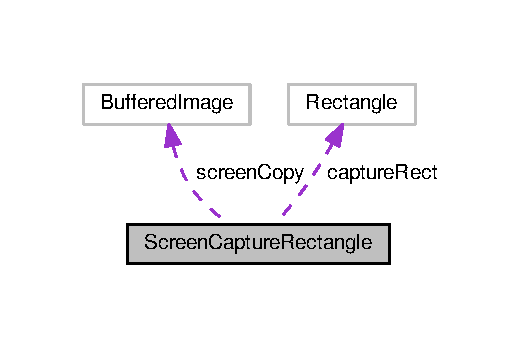
\includegraphics[width=255pt]{classScreenCaptureRectangle__coll__graph}
\end{center}
\end{figure}
\subsubsection*{Fonctions membres publiques}
\begin{DoxyCompactItemize}
\item 
void \hyperlink{classScreenCaptureRectangle_a2e065ce458964b134232f20e947d59aa}{repaint} (Buffered\+Image orig, Buffered\+Image copy)
\end{DoxyCompactItemize}
\subsubsection*{Fonctions membres publiques statiques}
\begin{DoxyCompactItemize}
\item 
static void \hyperlink{classScreenCaptureRectangle_ae7844603a26e5b4f73a3e023526c1a7e}{main} (String\mbox{[}$\,$\mbox{]} args)  throws Exception 
\end{DoxyCompactItemize}
\subsubsection*{Attributs publics}
\begin{DoxyCompactItemize}
\item 
Buffered\+Image \hyperlink{classScreenCaptureRectangle_a225d875cfde59bdcdb664be79d9ecd9c}{screen\+Copy}
\end{DoxyCompactItemize}
\subsubsection*{Fonctions de paquetage}
\begin{DoxyCompactItemize}
\item 
\hyperlink{classScreenCaptureRectangle_a9d00343f0ea876f310bcee635f9f49da}{Screen\+Capture\+Rectangle} (final Buffered\+Image screen)
\end{DoxyCompactItemize}
\subsubsection*{Attributs de paquetage}
\begin{DoxyCompactItemize}
\item 
Rectangle \hyperlink{classScreenCaptureRectangle_a0694872df9600fdd35dea40a88f4211f}{capture\+Rect}
\end{DoxyCompactItemize}


\subsubsection{Documentation des constructeurs et destructeur}
\hypertarget{classScreenCaptureRectangle_a9d00343f0ea876f310bcee635f9f49da}{}\index{Screen\+Capture\+Rectangle@{Screen\+Capture\+Rectangle}!Screen\+Capture\+Rectangle@{Screen\+Capture\+Rectangle}}
\index{Screen\+Capture\+Rectangle@{Screen\+Capture\+Rectangle}!Screen\+Capture\+Rectangle@{Screen\+Capture\+Rectangle}}
\paragraph[{Screen\+Capture\+Rectangle}]{\setlength{\rightskip}{0pt plus 5cm}Screen\+Capture\+Rectangle.\+Screen\+Capture\+Rectangle (
\begin{DoxyParamCaption}
\item[{final Buffered\+Image}]{screen}
\end{DoxyParamCaption}
)\hspace{0.3cm}{\ttfamily [package]}}\label{classScreenCaptureRectangle_a9d00343f0ea876f310bcee635f9f49da}


Référencé par main().



\subsubsection{Documentation des fonctions membres}
\hypertarget{classScreenCaptureRectangle_ae7844603a26e5b4f73a3e023526c1a7e}{}\index{Screen\+Capture\+Rectangle@{Screen\+Capture\+Rectangle}!main@{main}}
\index{main@{main}!Screen\+Capture\+Rectangle@{Screen\+Capture\+Rectangle}}
\paragraph[{main}]{\setlength{\rightskip}{0pt plus 5cm}static void Screen\+Capture\+Rectangle.\+main (
\begin{DoxyParamCaption}
\item[{String\mbox{[}$\,$\mbox{]}}]{args}
\end{DoxyParamCaption}
) throws Exception\hspace{0.3cm}{\ttfamily [static]}}\label{classScreenCaptureRectangle_ae7844603a26e5b4f73a3e023526c1a7e}
\hypertarget{classScreenCaptureRectangle_a2e065ce458964b134232f20e947d59aa}{}\index{Screen\+Capture\+Rectangle@{Screen\+Capture\+Rectangle}!repaint@{repaint}}
\index{repaint@{repaint}!Screen\+Capture\+Rectangle@{Screen\+Capture\+Rectangle}}
\paragraph[{repaint}]{\setlength{\rightskip}{0pt plus 5cm}void Screen\+Capture\+Rectangle.\+repaint (
\begin{DoxyParamCaption}
\item[{Buffered\+Image}]{orig, }
\item[{Buffered\+Image}]{copy}
\end{DoxyParamCaption}
)}\label{classScreenCaptureRectangle_a2e065ce458964b134232f20e947d59aa}


Référencé par Screen\+Capture\+Rectangle().



\subsubsection{Documentation des données membres}
\hypertarget{classScreenCaptureRectangle_a0694872df9600fdd35dea40a88f4211f}{}\index{Screen\+Capture\+Rectangle@{Screen\+Capture\+Rectangle}!capture\+Rect@{capture\+Rect}}
\index{capture\+Rect@{capture\+Rect}!Screen\+Capture\+Rectangle@{Screen\+Capture\+Rectangle}}
\paragraph[{capture\+Rect}]{\setlength{\rightskip}{0pt plus 5cm}Rectangle Screen\+Capture\+Rectangle.\+capture\+Rect\hspace{0.3cm}{\ttfamily [package]}}\label{classScreenCaptureRectangle_a0694872df9600fdd35dea40a88f4211f}
\hypertarget{classScreenCaptureRectangle_a225d875cfde59bdcdb664be79d9ecd9c}{}\index{Screen\+Capture\+Rectangle@{Screen\+Capture\+Rectangle}!screen\+Copy@{screen\+Copy}}
\index{screen\+Copy@{screen\+Copy}!Screen\+Capture\+Rectangle@{Screen\+Capture\+Rectangle}}
\paragraph[{screen\+Copy}]{\setlength{\rightskip}{0pt plus 5cm}Buffered\+Image Screen\+Capture\+Rectangle.\+screen\+Copy}\label{classScreenCaptureRectangle_a225d875cfde59bdcdb664be79d9ecd9c}


La documentation de cette classe a été générée à partir du fichier suivant \+:\begin{DoxyCompactItemize}
\item 
\hyperlink{oldCode_2ScreenCaptureRectangle_8java}{old\+Code/\+Screen\+Capture\+Rectangle.\+java}\end{DoxyCompactItemize}

%--- End generated contents ---

% Index
\newpage
\phantomsection
\addcontentsline{toc}{chapter}{Index}
\printindex

\end{document}
